\subsection{RAM access time}

\subsubsection{Estimation}

The RAM access time should access increasingly larger elements of the memory hierarchy as arrays grow bigger. We know from base hardware performance that smaller caches are faster than bigger ones, and CPU caches are faster to ask than main memory. The smallest arrays (<32kB) should access the L1 cache (onboard cache). The bigger arrays should access the L2 cache (<256kB). The even bigger arrays should access the L3 cache (<512kB). Finally the biggest arrays should access main memory (>3MB). We expect L1 cache access to be extremely fast (in the order of a few nanoseconds). We expect L2 cache access to be slightly more expensive  (less than a dozen nanoseconds). L3 cache should a few nanoseconds slower still. Finally, main memory should be significantly slower, because it would requires leaving the CPU and making a virtual address lookup. The LmBench paper provides a graphical representation of what we should expect as well.

\subsubsection{Methodology}

To measure RAM access time, we follow the methodology used in section 6.2 of the LmBench paper \cite{lmbench}. We create arrays of increasing sizes and iterate through them 1 000 000 times sequentially  (wrapping around if we reached the end of the array). Each such array is created at the beginning of an experiment and freed at the end. Thus, it has only one name, \texttt{array}. We also attempt different stride sizes. The contents of the arrays are filled as follows :

\begin{lstlisting}
for (int i = 0; i < size; i++)
  int cur_stride = i / stride;
  array[i] = (char*) &array
    [(cur_stride * stride +
    rand()\%stride) \% size];
\end{lstlisting}

where \texttt{stride} is the stride and \texttt{size} is the size of the array. Notice that we randomize the address of the next pointer within each stride.  We then traverse the array as follows :

\begin{lstlisting}
for (int i = 0; i < iterations; i++)
  for (int j = 0; j < stride_c; j++)
    char** p = (char**) array
       [stride_c * stride];
    // hundred times next stmt
    p = (char**) p;
\end{lstlisting}

where \texttt{stride\_c} is the number of strides within the array (always at least one). The \texttt{p = (char**) p} statement is loop enrolled a hundred time within each visit. Thanks to randomization, we minimize the effects of cache line prefetching. The size of the arrays created varies from 32KB ($2^{15}$) to 256MB ($2^{28}$). For each array size, strides 16,64,256 and 1024 are profiled. 

\subsubsection{Results}

The result of our experiment is shown on figure \ref{fig:b2blatency}. The resulting graph is similar to the one found in the LmBench paper. 

\begin{figure}
 \centering
  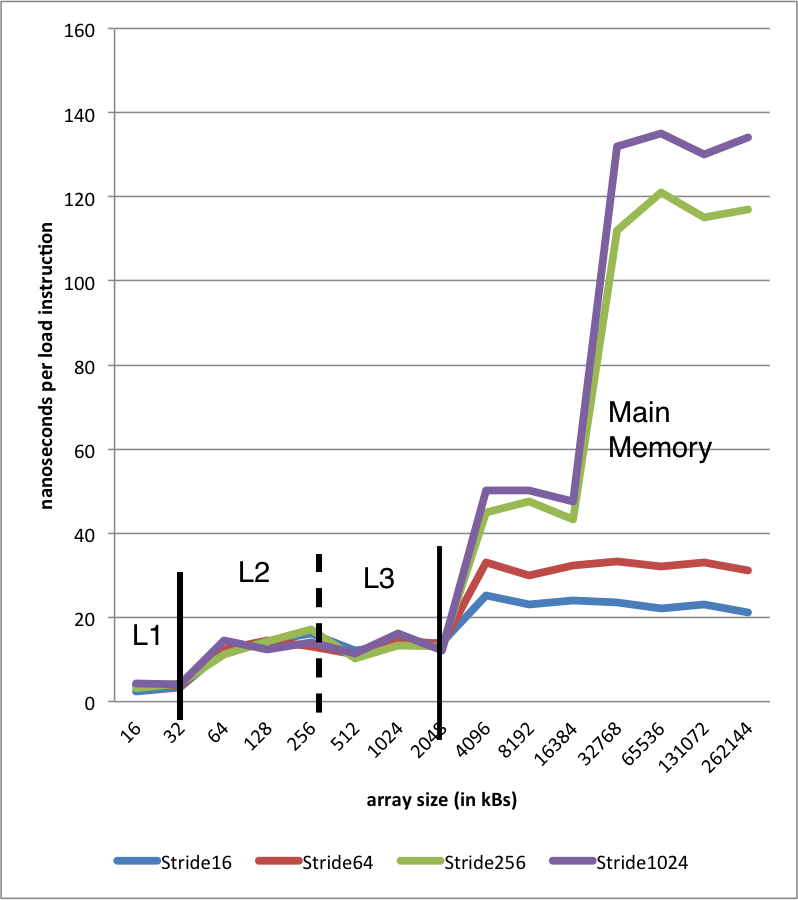
\includegraphics[width=0.5\textwidth]{image/backtobackload2.png}
  \caption{Back To Back Load Latency}
 \label{fig:b2blatency}
\end{figure}

\subsubsection{Analysis}

In terms hardware performance, our system has two 32kB L1 caches , 2 256kB L2 caches and 1 3MB L3 cache. From our vendor \cite{vendor}, we known that our cache lines are 128 bytes. The transition from L1 cache to L2 cache and L3 cache to main memory are clearly visible and follow what we would expect from our knowledge of the hardware. However, the transition from L2 cache to L3 cache isn't very noticeable. We are unable to compare with LMBench here because the computers profiled with LmBench do not have L3 caches. One possible reasoning is that the memory latency difference between the L2 and L3 cache is small and we suffer from small software overhead from looping through the strides and setting an initial value for \texttt{p}, which makes the transition indistinguishable. Finally, we also notice that when the stride size becomes greater than the cache line of the hardware, the main memory latency is greatly increased.

\subsection{RAM Bandwidth}

\subsubsection{Estimation}

RAM bandwidth metrics are provided by our vendor, which estimates it to 10GB/s for either reading or writing. In order to measure accurately our bandwidth we will need to use system calls to read or write large chunks of memory. For this purpose, we have chosen \texttt{memcpy}. However,  we will have to be careful about the software overhead incurred by such some system calls.
For example, in terms of software overhead, according to the LmBench paper, pure read represents only about one half to one third of the \texttt{memcpy} work. Therefore, we can expect read/width bandwidth to run at roughly twice the speed of a \texttt{memcpy} procedure call (assumption taken from the LmBench paper).

\subsubsection{Methodology}

To measure RAM bandwidth, we followed the methodology suggested by the LmBench paper. However, we used the \texttt{mempcy} function since the \texttt{bcopy} function used in the paper has been deprecated since.

For the read bandwidth, we created two arrays (of type \texttt{char}), called \texttt{bigArrayR} (162MB) and \texttt{smallArray} (3MB). \texttt{bigArray} is filled with random data before the beginning of the profiling (using \texttt{rand()}). When profiling starts, the contents of \texttt{bigArrayR} are sequentially read into \texttt{smallArray} in chunks of 3MB using \texttt{memcpy}  (in an enrolled loop).

The small array has been chosen to be exactly of the size of our L3 cache. After being repeatedly written into, it is expected that it will fill the contents of the cache, and all reads from \texttt{bigArrayR} are expected to originate from RAM.

Similarly for the write bandwidth, we keep \texttt{smallArray} and create a new empty array \texttt{bigArrayW} (162MB), left empty this time. When profiling starts, contents from \texttt{smallArray} are sequentially written into \texttt{bigArrayW} in chunks of 3MB using \texttt{memcpy} in an enrolled loop. After being repeatedly read from, it is expected that the contents of \texttt{smallArray} will fill the L3 cache, and all writes to \text{BigArrayW} will be written to RAM.

\subsubsection{Results}


We measure the time taken for reading the entire \texttt{bigArrayR} and write the entire \texttt{bigArrayW} (averaged over 5 runs). 
We obtain a raw read bandwidth of 4843 MB/sec and raw write bandwidth of 4612MB/sec using \texttt{memcpy}. We can expect our maximal read bandwidth to be between 9686 and 14529 MB/sec. Similarly, we can expect our write bandwidth to be between 9224 and 13836 MB/sec. Without understanding exactly what the \texttt{memcpy} procedure overhead is, we are unable to provide a more specific measurement.

\subsubsection{Analysis}

The results we have seem to concur the vendor's description, provided the software overhead estimate made for the \textt{memcpy} system call is accurate.

\subsection{Page Fault Service Time}

\subsubsection{Estimation}

\subsubsection{Methodology}

To profile page faults, we have used a mechanism proper to the Linux operating system called \textbf{Cgroups}. Cgroups are "tags" which can be specified when running process and which indicate to the operating system that only a restricted set of resources (indicated in the Cgroup description) should be allocated to the process. For example, we have restricted the amount of RAM used by the process for this experiment to 75MB.

In the experiment, we proceed to allocate an array (called \texttt{mallocs}) of 150 strings, each 1MB long. In order to ensure that the memory is actually allocated, we fill these 1MB strings with actual data. The memory allocation is done sequentially (the string for \texttt{mallocs[0]} is constructed before the string for \texttt{mallocs[1]} and so on...).

Given the process can only use 75MB of RAM, we can expect that at least half of the pages used by the \texttt{mallocs} array have been flushed to disk. Given data has been allocated sequentially, we can expect (according to the LRU rule), that these pages correspond to the first half of the array. The hardware performance of our SSD has been given by our vendor as a 520MB/sec read bandwidth. Software overhead is expected to be negligible in this experiment. However, in the context of a page fault, we can expect that after waiting for a while the OS might decide to do a context switch before coming back. Such context switch could occur while the process is waiting for a load instruction which is being profiled. As such, some fringe values in the experiment are to be expected as well.

\subsubsection{Results}

\begin{figure}
 \centering
  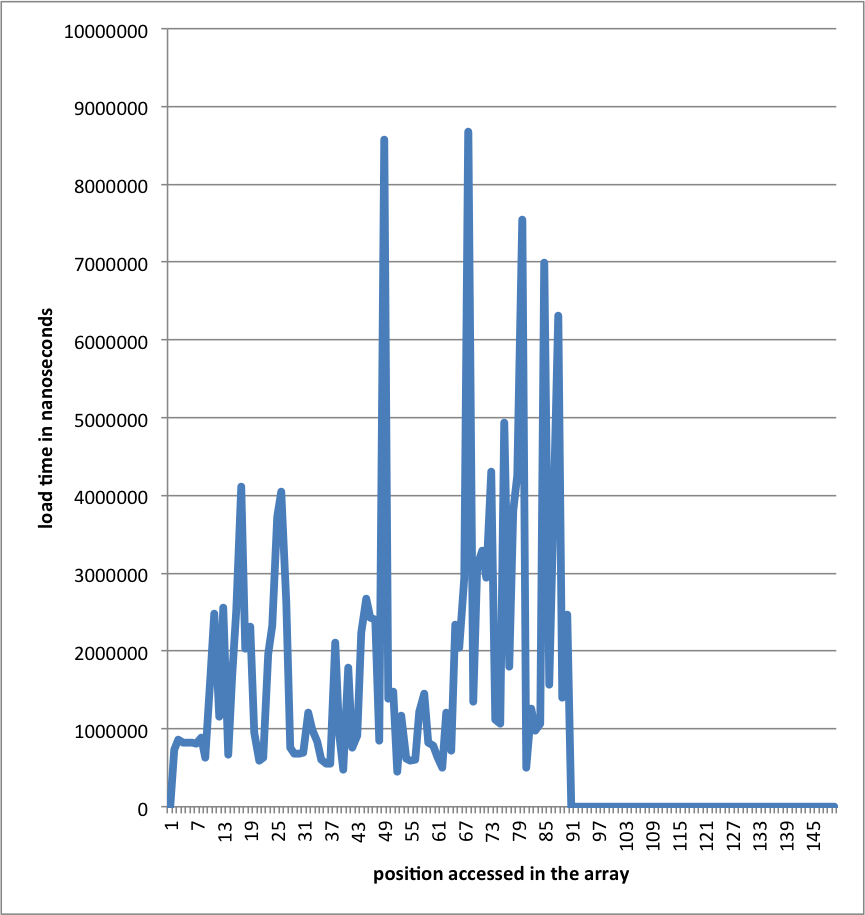
\includegraphics[width=0.5\textwidth]{image/pagefault.png}
  \caption{Page faults when accessing 150MB array}
 \label{fig:pagefault}
\end{figure}

These expectations are confirmed on figure ~\ref{fig:pagefault}. In this figure, we measure the time required to load each of the 1MB strings sequentially using \texttt{memcpy()} (we start by loading \texttt{mallocs[0]} and finish with \texttt{mallocs[149]}). We consider the 8-9 millisecond load times as the kind of fringe values we have to expect.
Given that the page size of our system is 4KB, 1MB corresponds to 256 pages. The median page load time for the first 90 MB is 1213/256 = 4.73  microseconds (which is consistent with the 750MB/sec bandwidth of our SSD). On the other hand, the average page load time for the last 60 MB is 0.8/256 = 0.00313  microseconds. This corresponds to a roughly 2000x increase when fetching pages from disk rather than main memory!

\subsubsection{Analysis}